\section{Modèle}

Le modèle que nous avons utilisé comporte 2 étapes:
\begin{enumerate}
 \item sélection des voxels les plus informatifs réalisée par un filtre univarié: voir~\autoref{subsec:filtre_univarie}
 \item classification à l'aide d'une régression logistique pénalisée: voir~\autoref{subsec:regression}
\end{enumerate}

Comme le modèle utilise une régression linéaire, un poids $\beta_i$ est associé à chaque voxel.
On peut donc obtenir une image des poids associé à chaque voxel (appelée carte des poids) qui permet de repérer des zones intervenant dans la classification, ce qui peut permettre de comprendre les processus biologiques à l'œuvre dans la maladie.

\subsection{Filtre univarié} \label{subsec:filtre_univarie}

On fait un test F de Fisher sur chaque voxel pour savoir si il prédit bien le statut clinique.
On sélectionne les $k$ meilleurs.

\subsection{Régression logistique pénalisée}  \label{subsec:regression}

% La régression linéaire consiste à calculer une droite qui passe au plus près de toutes les données en minimisant l'erreur.
% Cette erreur est représenté par la distance des données à la droite (la ligne verte sur le graphique)  (voir~\autoref{fig:regression_lineaire})
% 
% \begin{figure}[htpb]
% 	\centering
% 	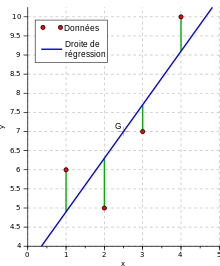
\includegraphics[scale = 0.5]{images/regression_lineaire}
% 	\caption{Graphique d'une régression linéaire classique}
% 	\label{fig:regression_lineaire}
% \end{figure}
%  
% les valeurs Y représente les résultats correspondant aux données de X et $\beta$ Les poids qui permettent de minimiser l'erreur de l'estimation, c'est à dire faire en sorte que la droite passe au plus prés possible de tous les points. 
% La formule de la régression linéaire est la suivante (à 1 dimension): 
% \begin{equation}
% Y = X * \beta + \epsilon
% \end{equation}
% $\epsilon$ est ici un nombre infiniment petit qui représente une variation minime sur tout estimateur car l'erreur est humaine et l'apprentissage aussi. 
% Cette formule nous permet facilement d'isoler $\beta$ afin de le calculer. 
% 
% En ce qui nous concerne, Y correspond à une matrice de dimension n ligne et une colonne. X représente une matrice de n ligne et p colonne ainsi $\beta$ représente une matrice à 1 ligne et p colonne. 
% Donc notre régression se calcul non pas sur une dimension mais sur n dimension. La formule devient donc :
% \begin{equation}
% Y = X_{1} * \beta_{1} +X_{2} * \beta_{2} + X_{3} * \beta_{3} + ... + \epsilon
% \end{equation}
% 
% 
% En nous basant sur cette formule, il est facile après d'isoler les $\beta_{i}$ et de les calculés. 

%Notre estimateur consiste à effectuer une régression logistique afin de trouver le vecteur de poids $\beta$ (ici, $\beta$ = $\theta$).
Dans un premier temps, une régression linéaire est effectuée et par dessus celle-ci, une fonction logistique est appliquée afin d'obtenir une classification binaire.

Afin d'éviter le problème de sur-apprentissage, ce modèle inclut 3 pénalités:
\begin{itemize}
 \item une pénalité sur la norme $\ell_1$ qui assure que peu de variables sont sélectionnées
 \item une pénalité sur la norme $\ell_2$ qui assure que les poids sont relativement faibles
 \item une pénalité sur la norme TV qui assure la continuité spatiale des poids  
\end{itemize}

La force de la pénalité est réglée par un hyper-paramètre.
En général, on fixe une pénalité globale $\alpha$ et des ratios $\alpha_{\ell_1}$, $\alpha_{\ell_2}$ et $\alpha_{TV}$ tels que:
\[
\alpha_{\ell_1} + \alpha_{\ell_2} + \alpha_{TV} = \alpha
\]

\subsection{Hyper-paramètres}

Le modèle a donc 4 hyper-paramètres:
\begin{enumerate}
 \item le nombre de voxels sélectionnés par le filtre univarié $k$
 \item la pénalité globale $\alpha$
 \item les ratio $\alpha_{TV}$ et $\alpha_{\ell_1}$ ($\alpha_{\ell_2}$ se déduisant automatiquement)
\end{enumerate}
